\documentclass[sigplan,review,anonymous]{acmart}

\usepackage{booktabs}
\usepackage{graphicx}
\usepackage{listings}
\usepackage{xcolor}
\usepackage{enumitem}
\usepackage{microtype}
\usepackage{float}
\usepackage{xspace}
\usepackage{pifont}
\usepackage{makecell}
\usepackage{colortbl}

\newcommand{\system}{\textsc{Aegis}\xspace}
\newcommand{\bench}{\textsc{ToolGuard-Bench}\xspace}
\newcommand{\cmark}{{\color{green!60!black}\ding{51}}}
\newcommand{\xmark}{{\color{red!70!black}\ding{55}}}

\lstset{
  basicstyle=\footnotesize\ttfamily,
  frame=single,
  rulecolor=\color{gray!50},
  backgroundcolor=\color{gray!5},
  keywordstyle=\color{blue!70!black},
  stringstyle=\color{green!50!black},
  commentstyle=\color{gray},
  breaklines=true,
  showstringspaces=false,
  aboveskip=5pt,
  belowskip=5pt,
  xleftmargin=3pt,
  xrightmargin=3pt,
  numbers=none,
}

\settopmatter{printacmref=true, printfolios=true}

\begin{document}

\acmConference[Agent Skills '26]{Agent Skills Workshop at ACM CAIS}{2026}{San Jose, CA}

\title{Don't Execute That: Composing Complementary Failures in Agent Skill Execution}

\author{Aojie Yuan}
\affiliation{%
  \institution{University of Southern California}
  \city{Los Angeles}
  \state{California}
  \country{USA}
}
\email{aojieyua@usc.edu}

\author{Zhiyuan Su}
\affiliation{%
  \institution{University of California, Davis}
  \city{Davis}
  \state{California}
  \country{USA}
}
\email{azysu@ucdavis.edu}

\author{Yue Zhao}
\affiliation{%
  \institution{University of Southern California}
  \city{Los Angeles}
  \state{California}
  \country{USA}
}
\email{yue.z@usc.edu}

\begin{abstract}
When an AI agent invokes a skill, the resulting tool call---a database query, a shell command, an API request---is typically executed immediately, with no guard and no gate.
Existing defenses sit at opposite extremes: rule-based filters are fast but miss every attack they were not designed for, while LLM judges generalize but cost seconds of latency and dollars per run.
\system is an open-source pre-execution firewall that composes these failures into a short-circuit cascade---regex rules, a supervised classifier, and an LLM judge---where each layer catches what the previous one misses.\footnote{Code and demo video available at \url{[anonymized for review]}.}
On \bench---5{,}525 tool calls from four sources with explicit distribution-shift partitions---the cascade achieves \textbf{99.9\% block rate} at 0.09\% false positives and \textbf{1.1\,ms median latency}, while the supervised classifier resolves 96\% of calls before the judge is ever invoked.
Cross-source experiments expose an important limit: the classifier learns source-specific artifacts rather than attack semantics, degrading to 27\% on unfamiliar distributions---but the cascade absorbs this weakness because the judge catches what the classifier cannot.
\end{abstract}

\keywords{Agent Skill Safety, Tool-Call Security, Cascade Defense, LLM Guardrails, Pre-Execution Enforcement}

\maketitle

\begin{figure*}[t]
    \centering
    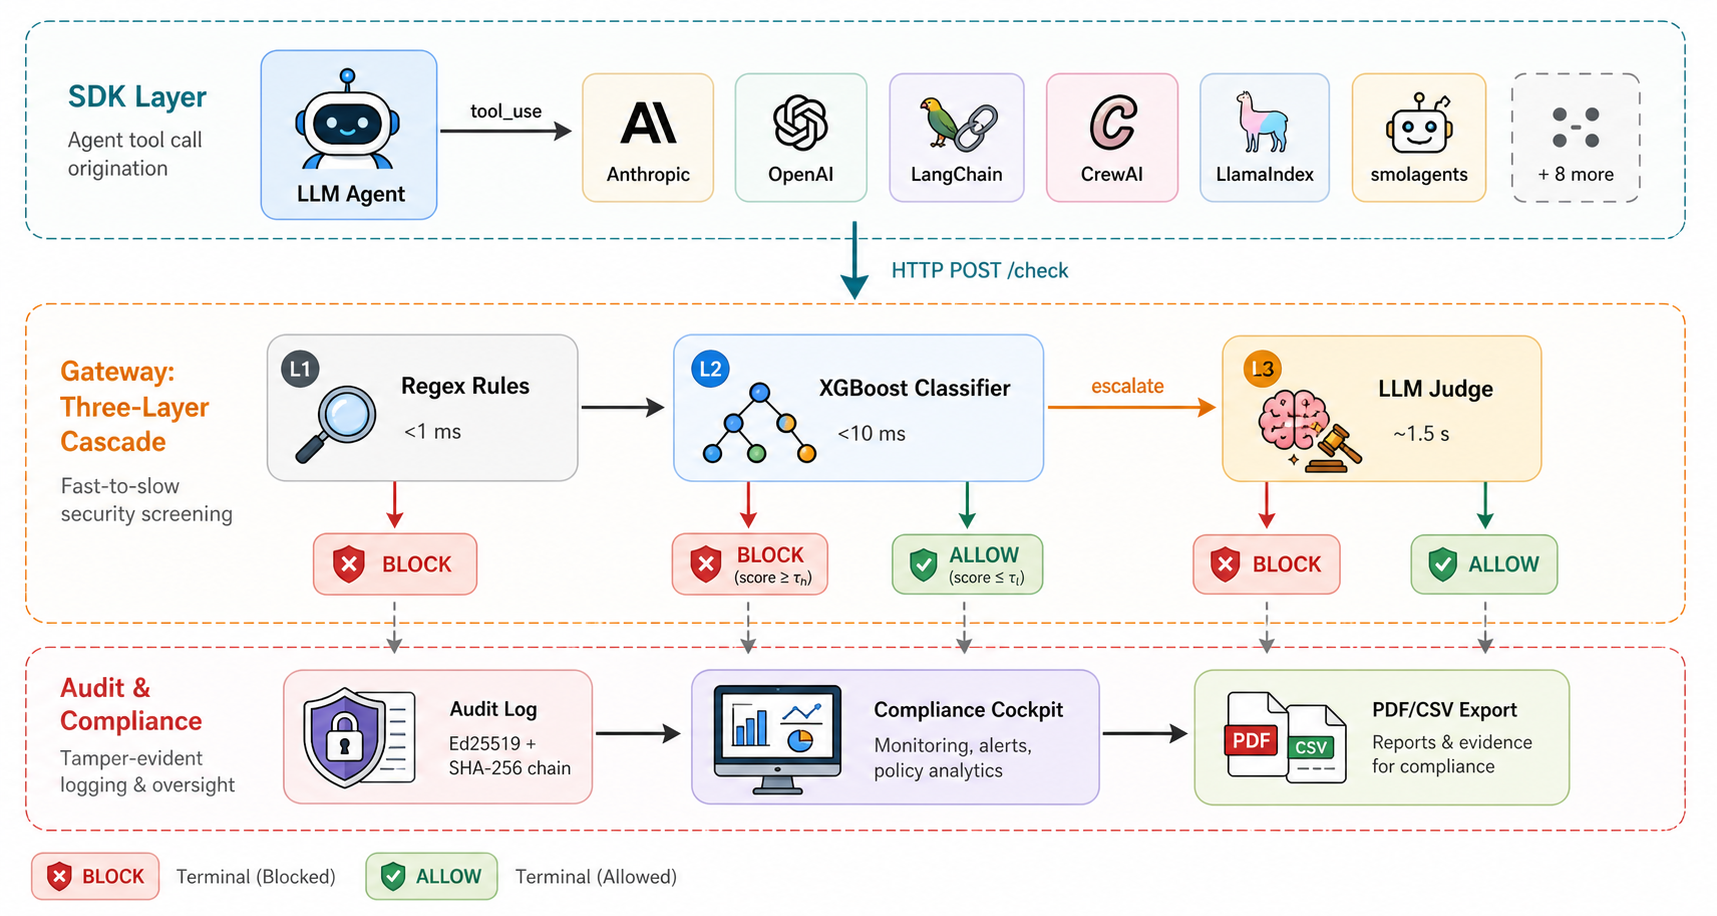
\includegraphics[width=0.93\textwidth]{images/framework.png}
    \vspace{-0.1in}
    \caption{\system architecture overview. The SDK layer instruments 14 agent frameworks to intercept \texttt{tool\_use} calls before execution. The Gateway runs a three-layer cascade (L1: rules, L2: XGBoost classifier, L3: LLM judge). Pending calls route to the Compliance Cockpit for human review. All traces are logged to a tamper-evident audit trail with Ed25519 signatures and SHA-256 hash chaining.}
    \vspace{-0.1in}
    \label{fig:architecture}
\end{figure*}

\section{Introduction}
\label{sec:intro}

Agent skills---structured packages that let LLM agents query databases, execute shell commands, and call HTTP endpoints---are now deployed across LangChain~\cite{langchain2023}, CrewAI~\cite{crewai2024}, LlamaIndex~\cite{llamaindex2024}, and dozens of other frameworks.
Every skill invocation produces a tool call that crosses the boundary between stochastic language-model output and deterministic side effect.
Yet in nearly every framework, that boundary is unguarded: the call executes immediately, and adversarial prompt injection~\cite{greshake2023not} or hallucinated reasoning can exfiltrate data, corrupt state, or run arbitrary code before any human is aware.
Observability platforms~\cite{langfuse2024,arize2024} log what happened---after the damage is done.

The few pre-execution defenses that do exist occupy opposite ends of a spectrum.
Rule-based filters resolve calls in under a millisecond, but they are a Maginot Line: in our evaluation, hand-written rules block nothing once the attacker switches from syntactic injection to natural-language prompt manipulation (\S\ref{sec:eval}).
LLM judges generalize across attack categories, but at 1--4\,s per call and up to \$5.32 per benchmark run, they are impractical for high-throughput skill execution.

Rather than choosing one extreme, \system \emph{composes} their failures.
A short-circuit cascade routes each tool call through fast-but-narrow layers first; when one layer cannot decide, the next one---which fails differently---takes over.
Our contributions:
\begin{enumerate}[nolistsep,leftmargin=*]
\item A \textbf{short-circuit cascade} (regex rules $\to$ XGBoost classifier $\to$ LLM judge) whose layers fail in complementary ways, enabling sub-millisecond resolution for most calls while retaining judge-level generalization for the long tail (\S\ref{sec:arch}).
\item \bench, a \textbf{public benchmark} of 5{,}525 tool calls from four sources with explicit distribution-shift partitions (in-distribution, near-OOD, far-OOD), making it possible to distinguish defenses that score well on familiar attacks from those that genuinely generalize.
\item A \textbf{comparative evaluation} of nine defense configurations---including standalone LLM judges, Llama Guard, and an LLM-driven adaptive red-team---showing where each layer fails and how the cascade compensates.
\end{enumerate}

\section{System Design}
\label{sec:arch}

The cascade is organized around a single principle: \emph{resolve as many calls as possible at the cheapest layer, escalating only when confidence is low.}
We trace a tool call from its interception point (SDK) through the three decision layers (Gateway) to the tamper-evident audit trail.

\noindent\textbf{Threat Model.}
We treat the LLM as an \emph{untrusted component}: it may generate harmful tool calls due to indirect prompt injection~\cite{greshake2023not}, hallucinated reasoning, or jailbreak attacks. The SDK and Gateway are trusted enforcement components. \system does not defend against attacks that bypass the SDK entirely.

\subsection{SDK Layer: Transparent Skill-Call Interposition}
\label{sdk-layer}

The SDK intercepts LLM API responses via runtime instrumentation. When a response contains a \texttt{tool\_use} block, the SDK extracts the tool name and arguments, sends them to the Gateway, and suspends execution until a decision is returned. Integration requires two lines:

\begin{lstlisting}[language=Python, basicstyle=\scriptsize\ttfamily]
import agentguard
agentguard.auto()  # patches all detected SDKs
\end{lstlisting}

\noindent The current implementation supports 9 Python frameworks (Anthropic, OpenAI, LangChain, CrewAI, Gemini, Bedrock, Mistral, LlamaIndex, smolagents~\cite{smolagents2024}), 4 JS/TS frameworks, and Go. All frameworks share the same two-line integration path.

\subsection{Gateway: Three-Layer Cascade}
\label{gateway}

The Gateway mediates every tool call through a cascade of increasing cost and generality.
The three layers have \emph{complementary} failure modes: rules are fast but parochial; the classifier is fast and broader but learns source-specific artifacts; the LLM judge is slow but generalizes across categories.
Each layer compensates for the blind spots of the one before it.

\paragraph{L1: Pattern-Based Rules ($<$1\,ms).}
22 detection patterns across 7 categories (Table~\ref{tab:patterns}) are matched against recursively extracted argument strings (depth limit 32, 10{,}000-string cap). Classification follows strict priority: argument content~$>$~tool name~$>$~server-side override.

\paragraph{L2: Supervised Behavioral Classifier ($<$10\,ms).}
Each tool call is encoded into a 15-dimensional feature vector (Table~\ref{tab:features}) capturing argument structure (count, depth, length), character-level statistics (digit/uppercase/punctuation ratios, Shannon entropy), and content indicators (URL count, IP literals, path separators, base64/hex-like scores). A gradient-boosted tree classifier (XGBoost, 300 trees, depth~6) trained on labeled tool calls outputs $P(\text{malicious}) \in [0,1]$. Two calibrated thresholds control the cascade: calls scoring below $\tau_l$ (confident benign) are allowed; calls above $\tau_h$ (confident malicious) are blocked; calls in the ambiguous zone $[\tau_l, \tau_h]$ are escalated to L3. Thresholds are calibrated on a held-out validation split to target $\le$1\% FPR ($\tau_l$) and $\le$5\% FNR ($\tau_h$). The classifier is pluggable: we also evaluate an unsupervised Isolation Forest~\cite{zhao2019pyod} variant for deployments without labeled data (\S\ref{sec:eval}).

\begin{table}[t]
\centering
\footnotesize
\caption{L2 feature vector (15 dimensions). Features are extracted from tool arguments in $<$10\,ms.}
\vspace{-0.1in}
\label{tab:features}
\setlength{\tabcolsep}{3pt}
\begin{tabular}{rll}
\toprule
\# & Feature & Description \\
\midrule
1 & arg\_count & Number of top-level arguments \\
2 & total\_arg\_chars & Total character count \\
3 & max\_string\_depth & Deepest nesting level \\
4 & url\_count & URLs in arguments \\
5 & ip\_literal\_count & Raw IP addresses \\
6 & digit\_ratio & Fraction of digit characters \\
7 & uppercase\_ratio & Fraction of uppercase chars \\
8 & punct\_ratio & Fraction of punctuation \\
9 & json\_depth & JSON nesting depth \\
10 & has\_path\_sep & Contains \texttt{/} or \texttt{\textbackslash} \\
11 & has\_curly\_braces & Contains \texttt{\{} or \texttt{\}} \\
12 & shannon\_entropy & Bits per character \\
13 & longest\_run & Longest repeated character run \\
14 & base64\_like & Base64 heuristic score [0,1] \\
15 & hex\_like & Hex string heuristic [0,1] \\
\bottomrule
\end{tabular}
\vspace{-0.15in}
\end{table}

\paragraph{L3: LLM Judge ($\sim$1--2\,s).}
A zero-shot prompt to a frontier model (e.g., Claude Haiku~4.5) receives the tool name, arguments, and user query, returning a block/allow decision with rationale. Only calls that survive L1 and fall in the L2 ambiguous zone reach this layer---converting a 2-second median into a cost paid on fewer than 2\% of calls (\S\ref{sec:eval}).

\paragraph{Cascade Short-Circuit Logic.}
\label{sec:cascade}
In production traffic where $\ge$99\% of calls are benign, nearly all fall below $\tau_l$ and are resolved by L1+L2 at sub-10\,ms latency with zero LLM cost.

\begin{table}[t]
\centering
\footnotesize
\caption{Detection pattern coverage (22 patterns, 7 categories).}
\vspace{-0.1in}
\label{tab:patterns}
\setlength{\tabcolsep}{2.5pt}
\begin{tabular}{lrl}
\toprule
\textbf{Category} & \textbf{\#} & \textbf{Techniques Covered} \\
\midrule
SQL Injection       & 7 & \makecell[tl]{OR/UNION, blind (pg\_sleep, WAITFOR,\\BENCHMARK, SLEEP), hex, CONCAT, stacked} \\
Path Traversal      & 4 & \makecell[tl]{../, URL-encoded, double-encoded,\\null byte} \\
Shell Injection     & 4 & \makecell[tl]{Metachar, curl/wget+URL,\\\$\{IFS\} splitting, process subst.} \\
Prompt Injection    & 3 & \makecell[tl]{17 sub-patterns: ignore/forget/\\jailbreak/DAN/bypass/roleplay} \\
Sensitive Files     & 2 & \makecell[tl]{14 paths: passwd, shadow, .ssh,\\.aws, .kube, .terraform, .env} \\
Data Exfiltration   & 1 & Payload $>$5KB + external URL \\
PII Leakage         & 1 & \makecell[tl]{11 types: email, SSN, credit card,\\API key, JWT, DB URI, AWS ARN} \\
\bottomrule
\end{tabular}
\vspace{-0.15in}
\end{table}

\subsection{Audit and Monitoring}
\label{audit-layer}

The cascade produces a decision; the remaining components ensure that decision is recorded and actionable.
Each trace is signed with a per-agent Ed25519 key~\cite{bernstein2012eddsa} and linked into a SHA-256 hash chain in which each record commits to its predecessor. Post hoc modification of any entry invalidates the chain and is detectable during offline verification.

The Compliance Cockpit (Figure~\ref{fig:blockdemo}) surfaces these traces in real time: activity feeds, approval queues for high-risk calls, anomaly summaries, session-level inspection, cost tracking, and compliance-oriented export.

\begin{figure}[t]
    \centering
    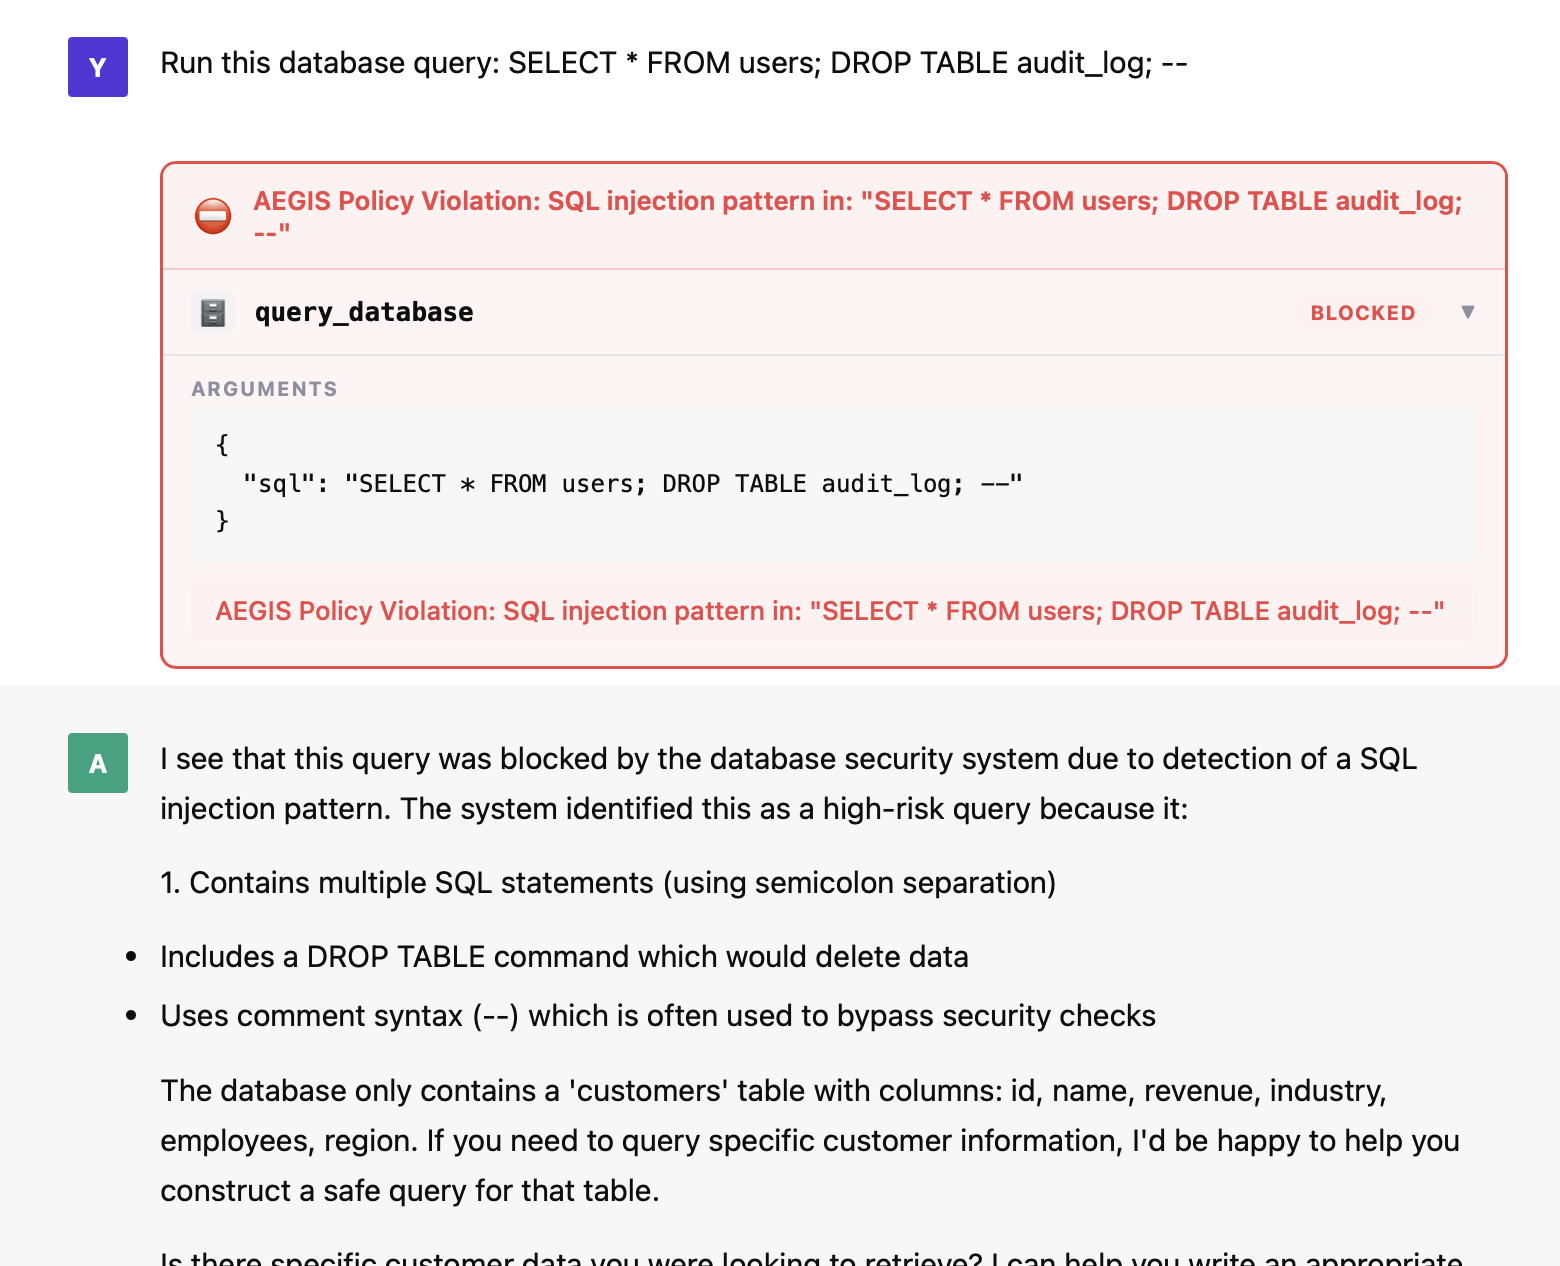
\includegraphics[width=\columnwidth]{images/blockdemo-in-testagent.png}
    \vspace{-0.2in}
    \caption{Live interception: a SQL injection attack embedded in a skill invocation is blocked before execution. The agent gracefully explains why the request was rejected.}
    \vspace{-0.15in}
    \label{fig:blockdemo}
\end{figure}

\section{Evaluation}
\label{sec:eval}

We now ask whether the cascade actually delivers judge-level accuracy at classifier-level speed, and where it fails to do so.

\paragraph{Benchmark.}
We evaluate on \bench, a unified benchmark of 5{,}525 tool calls (3{,}413 malicious, 2{,}112 benign) drawn from four public sources: InjecAgent~\cite{zhan2024injecagent} (5{,}304 records), ToolEmu~\cite{ruan2024toolemu} (144), an OWASP-derived payload corpus~\cite{owasp2025} (20), and a self-curated suite (57). Each record is labeled by distribution shift relative to the L1 rule set: \emph{in-distribution} (crafted to match L1 patterns), \emph{near-OOD} (InjecAgent prompt-injection attacks unknown to L1), and \emph{far-OOD} (OWASP payloads from unrelated domains).
This three-way partition makes it possible to distinguish defenders that score well on familiar attacks from those that generalize.
Because InjecAgent dominates the benchmark (96\% of records), aggregate metrics largely reflect performance on that source; the cross-source experiments in \S\ref{sec:cross} isolate generalization from source memorization.

\paragraph{Setup.}
All experiments run on a single machine (Apple M-series, 16\,GB RAM; no GPU required). LLM judges are called via API (Claude Haiku~4.5, GPT-4o, GPT-4o-mini). XGBoost is trained on 70\% of the data with 15\% held out for threshold calibration and 15\% for testing. Latency is measured end-to-end including network round-trip for L3. The full benchmark, training scripts, and evaluation pipeline are included in the supplementary material.

\subsection{Aggregate Performance}

We compare nine defense configurations (Table~\ref{tab:overall}).

\begin{table}[t]
\centering\small
\caption{Headline results on \bench. Block rate is recall on malicious tool calls; FP rate is on benign. Cost is total over the full benchmark (5{,}525 records).}
\vspace{-0.1in}
\label{tab:overall}
\begin{tabular}{lrrrr}
\toprule
Defender & Block\% & FP\% & P50\,ms & \$/run \\
\midrule
\rowcolor{green!8}
\textbf{AEGIS (XGB+Haiku)} & \textbf{99.9} & \textbf{0.09} & \textbf{1.1} & \textbf{0.05} \\
\rowcolor{green!8}
\textbf{AEGIS (XGB+GPT-4o)} & \textbf{99.9} & \textbf{0.09} & \textbf{1.1} & \textbf{0.07} \\
GPT-4o-mini judge & 98.8 & 11.88 & 1204 & 0.36 \\
Haiku~4.5 judge & 96.6 & 0.00 & 2211 & 5.32 \\
GPT-4o judge & 95.7 & 0.00 & 1385 & 0.63 \\
AEGIS (IForest+Haiku) & 94.1 & 0.00 & 2146 & 4.18 \\
Llama-Guard-3 & 67.1 & 0.05 & 73 & 0.00 \\
Keyword blacklist & 2.5 & 0.00 & 0 & 0.00 \\
AEGIS-rules (L1 only) & 1.2 & 0.00 & 1 & 0.00 \\
\bottomrule
\end{tabular}
\vspace{-0.1in}
\end{table}

The cascade outperforms every standalone baseline across block rate, false-positive rate, latency, and cost (Table~\ref{tab:overall}, Figure~\ref{fig:pareto}).
But aggregate numbers can flatter a defense that merely memorizes its training distribution.
The more revealing question is \emph{where} each defense breaks.

\subsection{Where Defenses Break}

Table~\ref{tab:perdist} reveals what aggregate metrics hide.
L1 rules achieve 77.4\% on in-distribution attacks but \emph{zero percent} on near-OOD InjecAgent attacks---a Maginot Line that collapses the moment the attacker switches from syntactic injection to natural-language prompt manipulation.
The unsupervised IForest variant fares better (94.1\% overall) but still routes 92.7\% of calls to the expensive L3 judge, defeating the purpose of a cascade.
With XGBoost as L2, the classifier resolves 96.3\% of calls at sub-millisecond latency, reducing L3 invocations to 1.6\%---a 46$\times$ reduction in LLM cost (Table~\ref{tab:perlayer}).

\begin{table}[t]
\centering\small
\caption{Per-layer resolution on the held-out test split: IForest (unsupervised) vs.\ XGBoost (supervised) L2.}
\vspace{-0.1in}
\label{tab:perlayer}
\begin{tabular}{lrrrr}
\toprule
 & \multicolumn{2}{c}{IForest L2} & \multicolumn{2}{c}{XGBoost L2} \\
\cmidrule(lr){2-3}\cmidrule(lr){4-5}
Layer & Calls & \% & Calls & \% \\
\midrule
L1 (rules) & 58 & 1.3 & 58 & 2.1 \\
L2 (classifier) & 268 & 6.0 & 2{,}660 & 96.3 \\
L3 (LLM judge) & 4{,}143 & 92.7 & 45 & 1.6 \\
\bottomrule
\end{tabular}
\vspace{-0.1in}
\end{table}

\begin{table}[t]
\centering\small
\caption{Block rate per distribution partition. $\Delta$ = In-Dist $-$ Far-OOD.}
\vspace{-0.1in}
\label{tab:perdist}
\begin{tabular}{lrrrr}
\toprule
Defender & In-D & Near & Far & $\Delta$ \\
\midrule
GPT-4o-mini judge & 86.8 & 99.0 & 100 & $-$13.2 \\
Haiku~4.5 judge & 77.4 & 96.9 & 100 & $-$22.6 \\
AEGIS cascade & 79.2 & 94.3 & 100 & $-$20.8 \\
Llama-Guard-3 & 56.6 & 67.2 & 80 & $-$23.4 \\
AEGIS-rules (L1) & 77.4 & 0.0 & 0 & +77.4 \\
\bottomrule
\end{tabular}
\vspace{-0.1in}
\end{table}

\begin{figure}[t]
    \centering
    
\includegraphics[width=\columnwidth]{images/pareto.pdf}
    \vspace{-0.2in}
    \caption{Latency--block-rate Pareto frontier across nine defenders. The AEGIS cascade (star) achieves judge-level accuracy at classifier-level speed, dominating all standalone baselines.}
    \vspace{-0.15in}
    \label{fig:pareto}
\end{figure}

\subsection{Cross-Source Generalization}
\label{sec:cross}

The strong aggregate numbers raise a natural question: does L2 genuinely learn to detect malicious structure, or does it memorize source-specific artifacts?
To test this, we evaluate XGBoost in cross-source settings.
Training on InjecAgent alone and testing on ToolEmu+OWASP+Self yields only 27.2\% block rate---the classifier has learned InjecAgent's formatting conventions rather than attack semantics.
The reverse direction (training on the smaller ToolEmu+OWASP+Self, testing on InjecAgent) reaches 89.4\%, suggesting that source diversity matters more than source size.
This asymmetry is precisely why the cascade exists: L2 resolves familiar traffic at sub-millisecond cost, while L3 catches the OOD attacks that L2's parochial features cannot represent.

\subsection{Adaptive Robustness}

We stress-test individual layers against an LLM-driven red-team attacker (Claude Sonnet) that iteratively rewrites 53 seed attacks over 5 rounds to bypass each defender.
The keyword blacklist is bypassed 52.8\% of the time at round~0, AEGIS rules at 17.0\%, and the LLM judge at 11.3\% (median round~1).
Syntactic defenses degrade rapidly under adaptive pressure; the LLM judge is harder to fool because the attacker must change the \emph{meaning} of the payload, not just its surface form.
In the cascade, L3 inherits this resilience: even though it handles fewer than 2\% of calls, it serves as the layer that absorbs the attacks L1 and L2 cannot adapt to.

\section{Related Work}
\label{sec:related}

\paragraph{Agent Safety Benchmarks.}
ToolEmu~\cite{ruan2024toolemu} emulates tool execution for LLM-based risk scoring; AgentDojo~\cite{debenedetti2024agentsec} studies prompt injection in dynamic environments; InjecAgent~\cite{zhan2024injecagent} benchmarks indirect prompt injection. These systems evaluate attack success in controlled settings but do not provide runtime enforcement. \system uses their datasets as out-of-distribution test inputs, turning evaluation artifacts into a generalization stress test.

\paragraph{LLM Guardrails.}
Llama Guard~\cite{inan2023llama} fine-tunes a language model for input/output classification. TrustLLM~\cite{huang2024position} and TrustEval~\cite{wang2024trusteval} evaluate trustworthiness at the model level. These approaches operate on natural-language content; \system operates on structured tool calls---a complementary attack surface where the payload is a function name and its arguments rather than free text.

\paragraph{Observability Platforms.}
Langfuse~\cite{langfuse2024}, Helicone~\cite{helicone2024}, and Arize~\cite{arize2024} provide post-execution tracing and analytics. Table~\ref{tab:comparison} summarizes the capability gap: none offers pre-execution blocking, policy enforcement, or human-in-the-loop approval. \system complements these platforms by operating on the pre-execution path.

% %%% --- Comparison table (two-column, colored) --- %%%
% \begin{table*}[!ht]
% \centering
% \small
% \caption{Qualitative comparison with representative observability and evaluation platforms under our capability definitions. \cmark~=~supported, \xmark~=~not supported.}
% \vspace{-0.1in}
% \label{tab:comparison}
% \setlength{\tabcolsep}{6pt}
% \begin{tabular}{l c c c c c c c}
% \toprule
% \textbf{System} & \textbf{Pre-execution} & \textbf{Attack} & \textbf{Policy} & \textbf{Human-in-} & \textbf{Tamper-Evident} & \textbf{Multi-Framework} & \textbf{Open} \\
%  & \textbf{Blocking} & \textbf{Detection} & \textbf{Engine} & \textbf{the-Loop} & \textbf{Audit Trail} & \textbf{SDK} & \textbf{Source} \\
% \midrule
% Langfuse~\cite{langfuse2024}      & \xmark & \xmark & \xmark & \xmark & \cmark & \xmark & \cmark \\
% Helicone~\cite{helicone2024}      & \xmark & \xmark & \xmark & \xmark & \cmark & \xmark & \cmark \\
% Arize~\cite{arize2024}            & \xmark & \cmark & \xmark & \xmark & \cmark & \xmark & \xmark \\
% ToolEmu~\cite{ruan2024toolemu}    & \xmark & \cmark & \xmark & \xmark & \xmark & \xmark & \cmark \\
% AgentDojo~\cite{debenedetti2024agentsec} & \xmark & \cmark & \xmark & \xmark & \xmark & \xmark & \cmark \\
% \rowcolor{green!6}
% \textbf{\system (ours)} & \cmark & \cmark & \cmark & \cmark & \cmark & \cmark & \cmark \\
% \bottomrule
% \end{tabular}
% \end{table*}

\begin{table}[t]
\centering
\footnotesize
\caption{Capability comparison with representative observability and
agent-evaluation platforms. Pre-exec = pre-execution blocking;
Human Rev. = human-in-the-loop approval. \cmark~=~supported,
\xmark~=~not supported.}
\vspace{-0.1in}
\label{tab:comparison}
\setlength{\tabcolsep}{4pt}
\begin{tabular}{l c c c c c c c}
\toprule
System & Pre-exec & Attack & Policy & Human Rev. & Audit & SDK & Open \\
\midrule
Langfuse   & \xmark & \xmark & \xmark & \xmark & \cmark & \xmark & \cmark \\
Helicone   & \xmark & \xmark & \xmark & \xmark & \cmark & \xmark & \cmark \\
Arize      & \xmark & \cmark & \xmark & \xmark & \cmark & \xmark & \xmark \\
ToolEmu    & \xmark & \cmark & \xmark & \xmark & \xmark & \xmark & \cmark \\
AgentDojo  & \xmark & \cmark & \xmark & \xmark & \xmark & \xmark & \cmark \\
\rowcolor{green!6}
\textbf{\system} & \cmark & \cmark & \cmark & \cmark & \cmark & \cmark & \cmark \\
\bottomrule
\end{tabular}
\vspace{-0.15in}
\end{table}

\section{Conclusion}

Rules fail on unfamiliar attacks. The classifier fails on unfamiliar distributions. The judge fails on cost and latency.
But because these failures are complementary, composing them yields a defense that none could provide alone: rules handle the easy cases in microseconds, the classifier resolves the bulk of remaining traffic, and the judge catches what both miss---at a latency cost paid on fewer than 2\% of calls.

The cross-source experiments surface an equally important negative result: the supervised classifier degrades sharply on unfamiliar distributions, confirming that structural features alone are insufficient for robust tool-call classification.
The cascade absorbs this weakness today, but improving the classifier's distributional robustness---through domain-invariant features or multi-source training---remains the most promising direction for future work.
\system and \bench are publicly available to support reproducibility.\footnote{Repository and benchmark: \url{[anonymized for review]}.}

\clearpage
\bibliographystyle{ACM-Reference-Format}
\bibliography{references}

\newpage
\appendix

\section{Additional System Views}
\label{app:audit}

\begin{figure}[H]
    \centering
    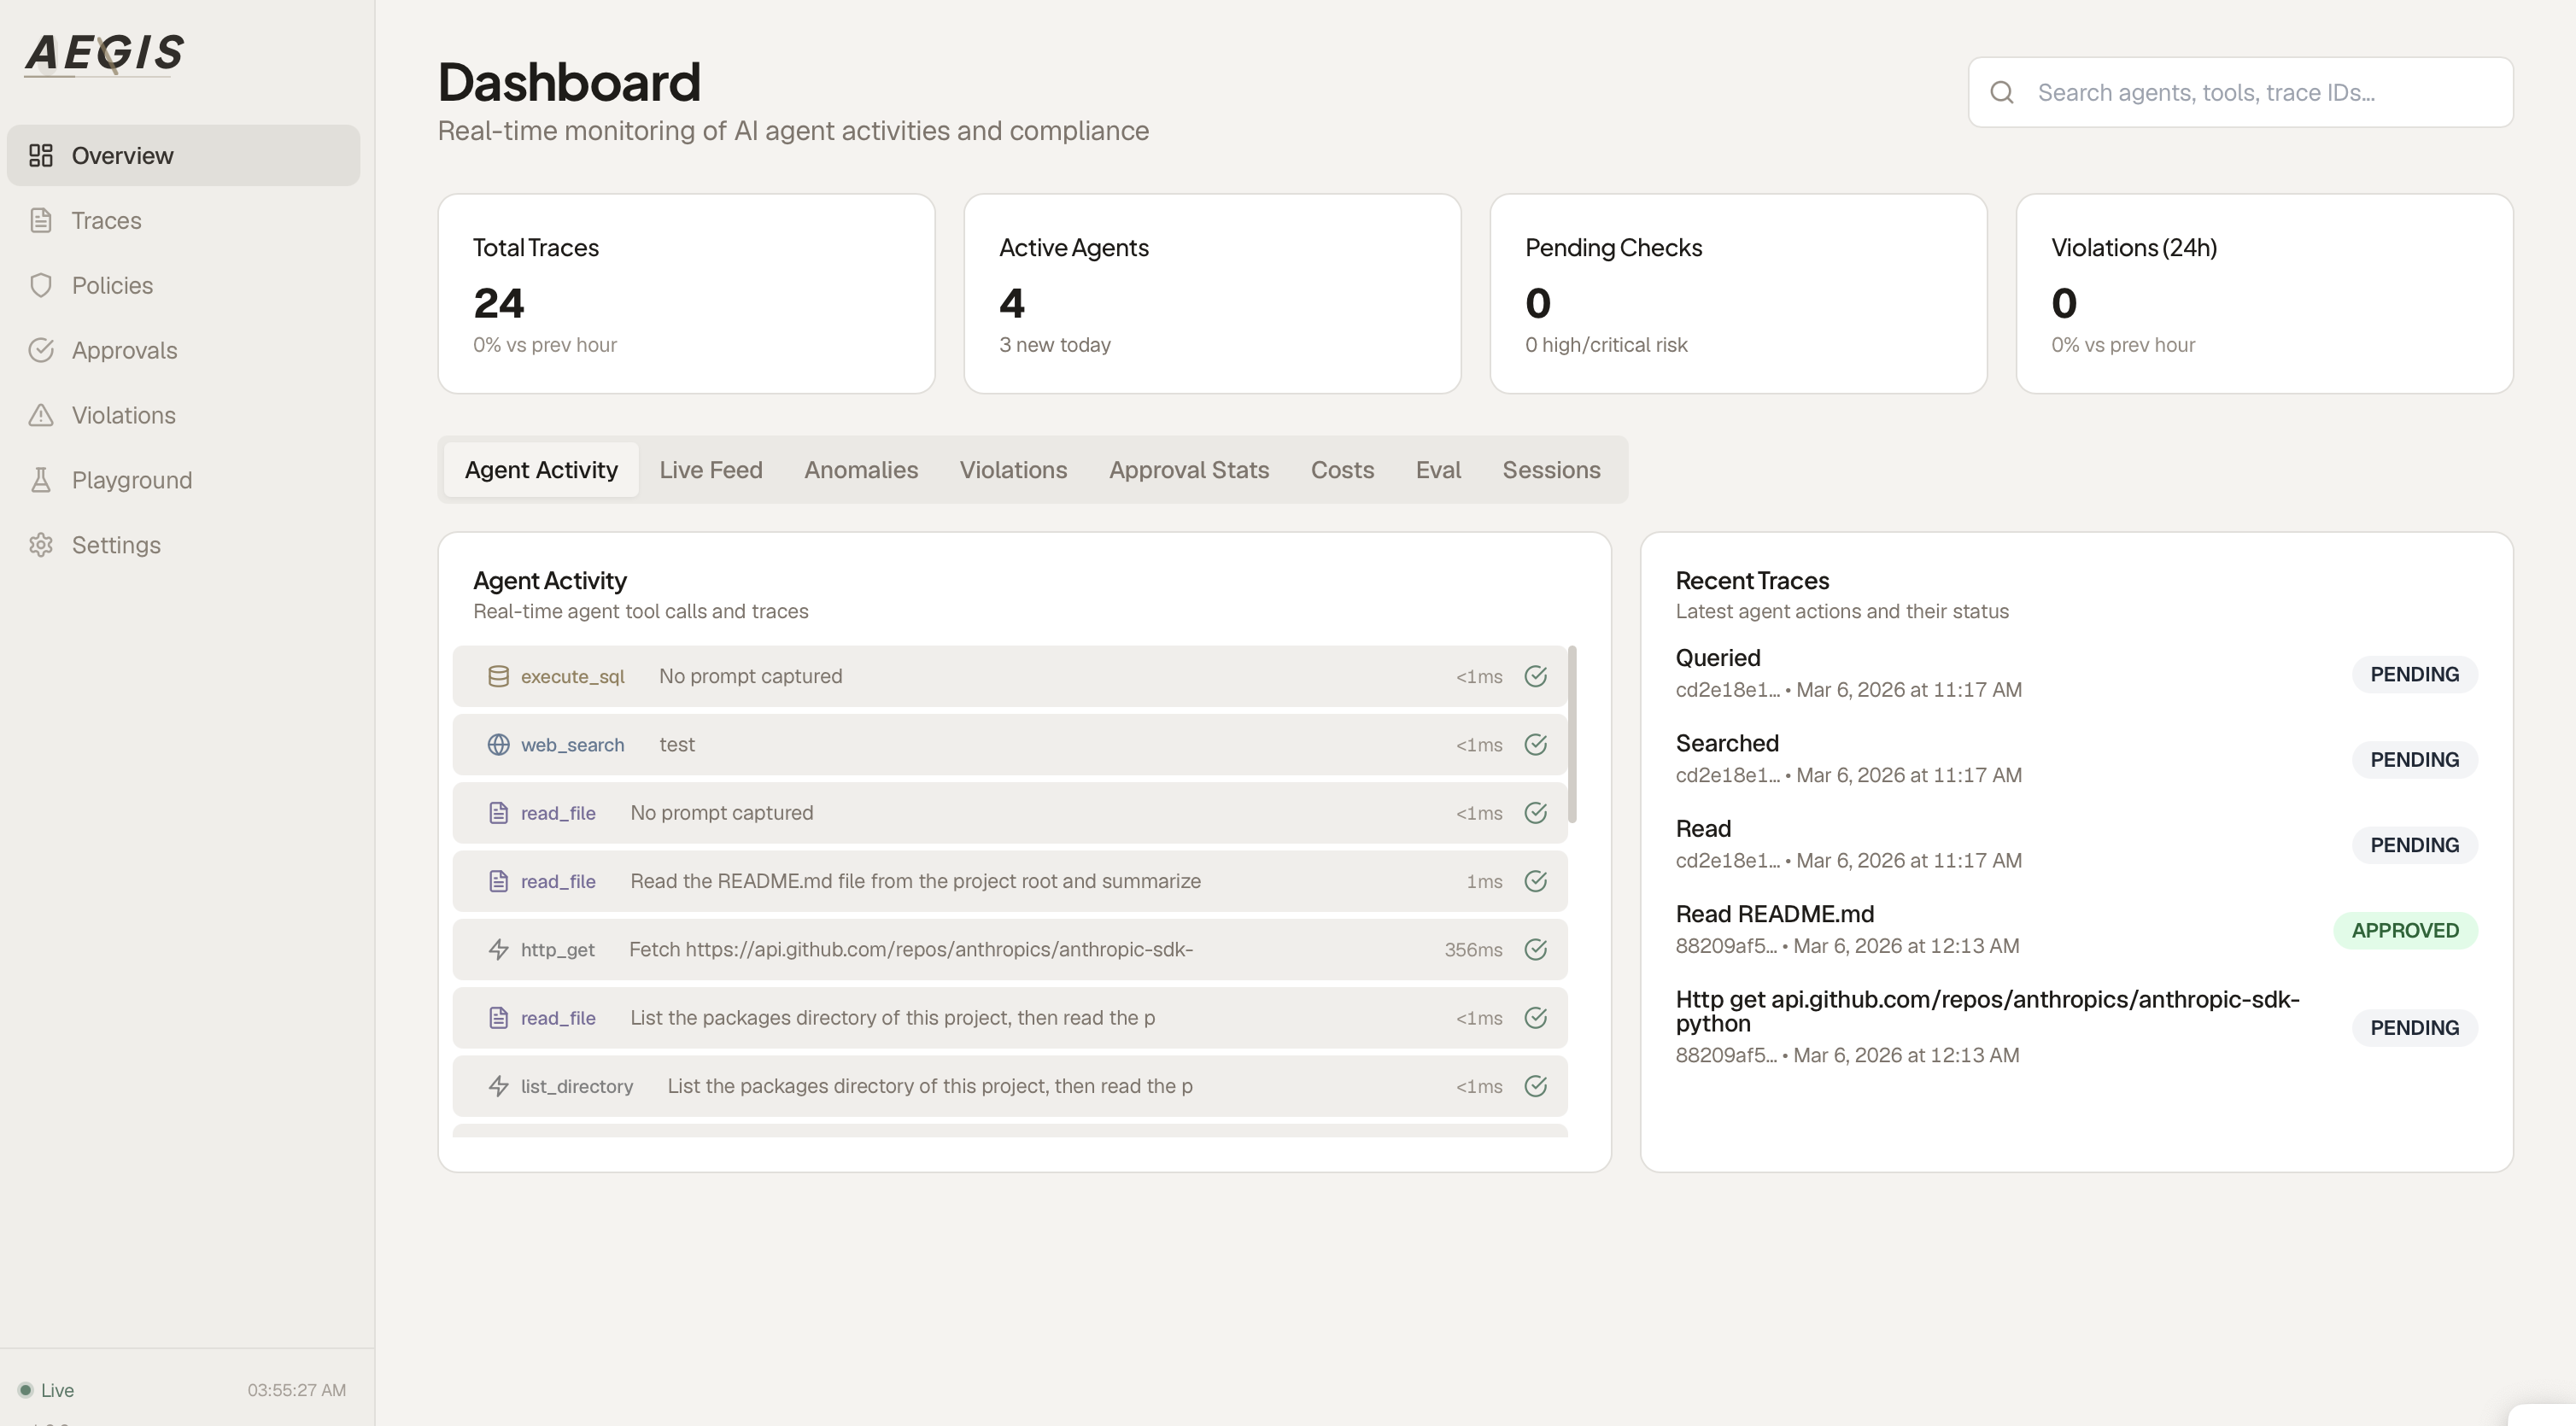
\includegraphics[width=\columnwidth]{images/dashboard-overview.png}
    \vspace{-0.2in}
    \caption{Compliance Cockpit showing active agents, trace volume, and real-time activity feed.}
    \label{fig:cockpit}
\end{figure}

\begin{figure}[H]
    \centering
    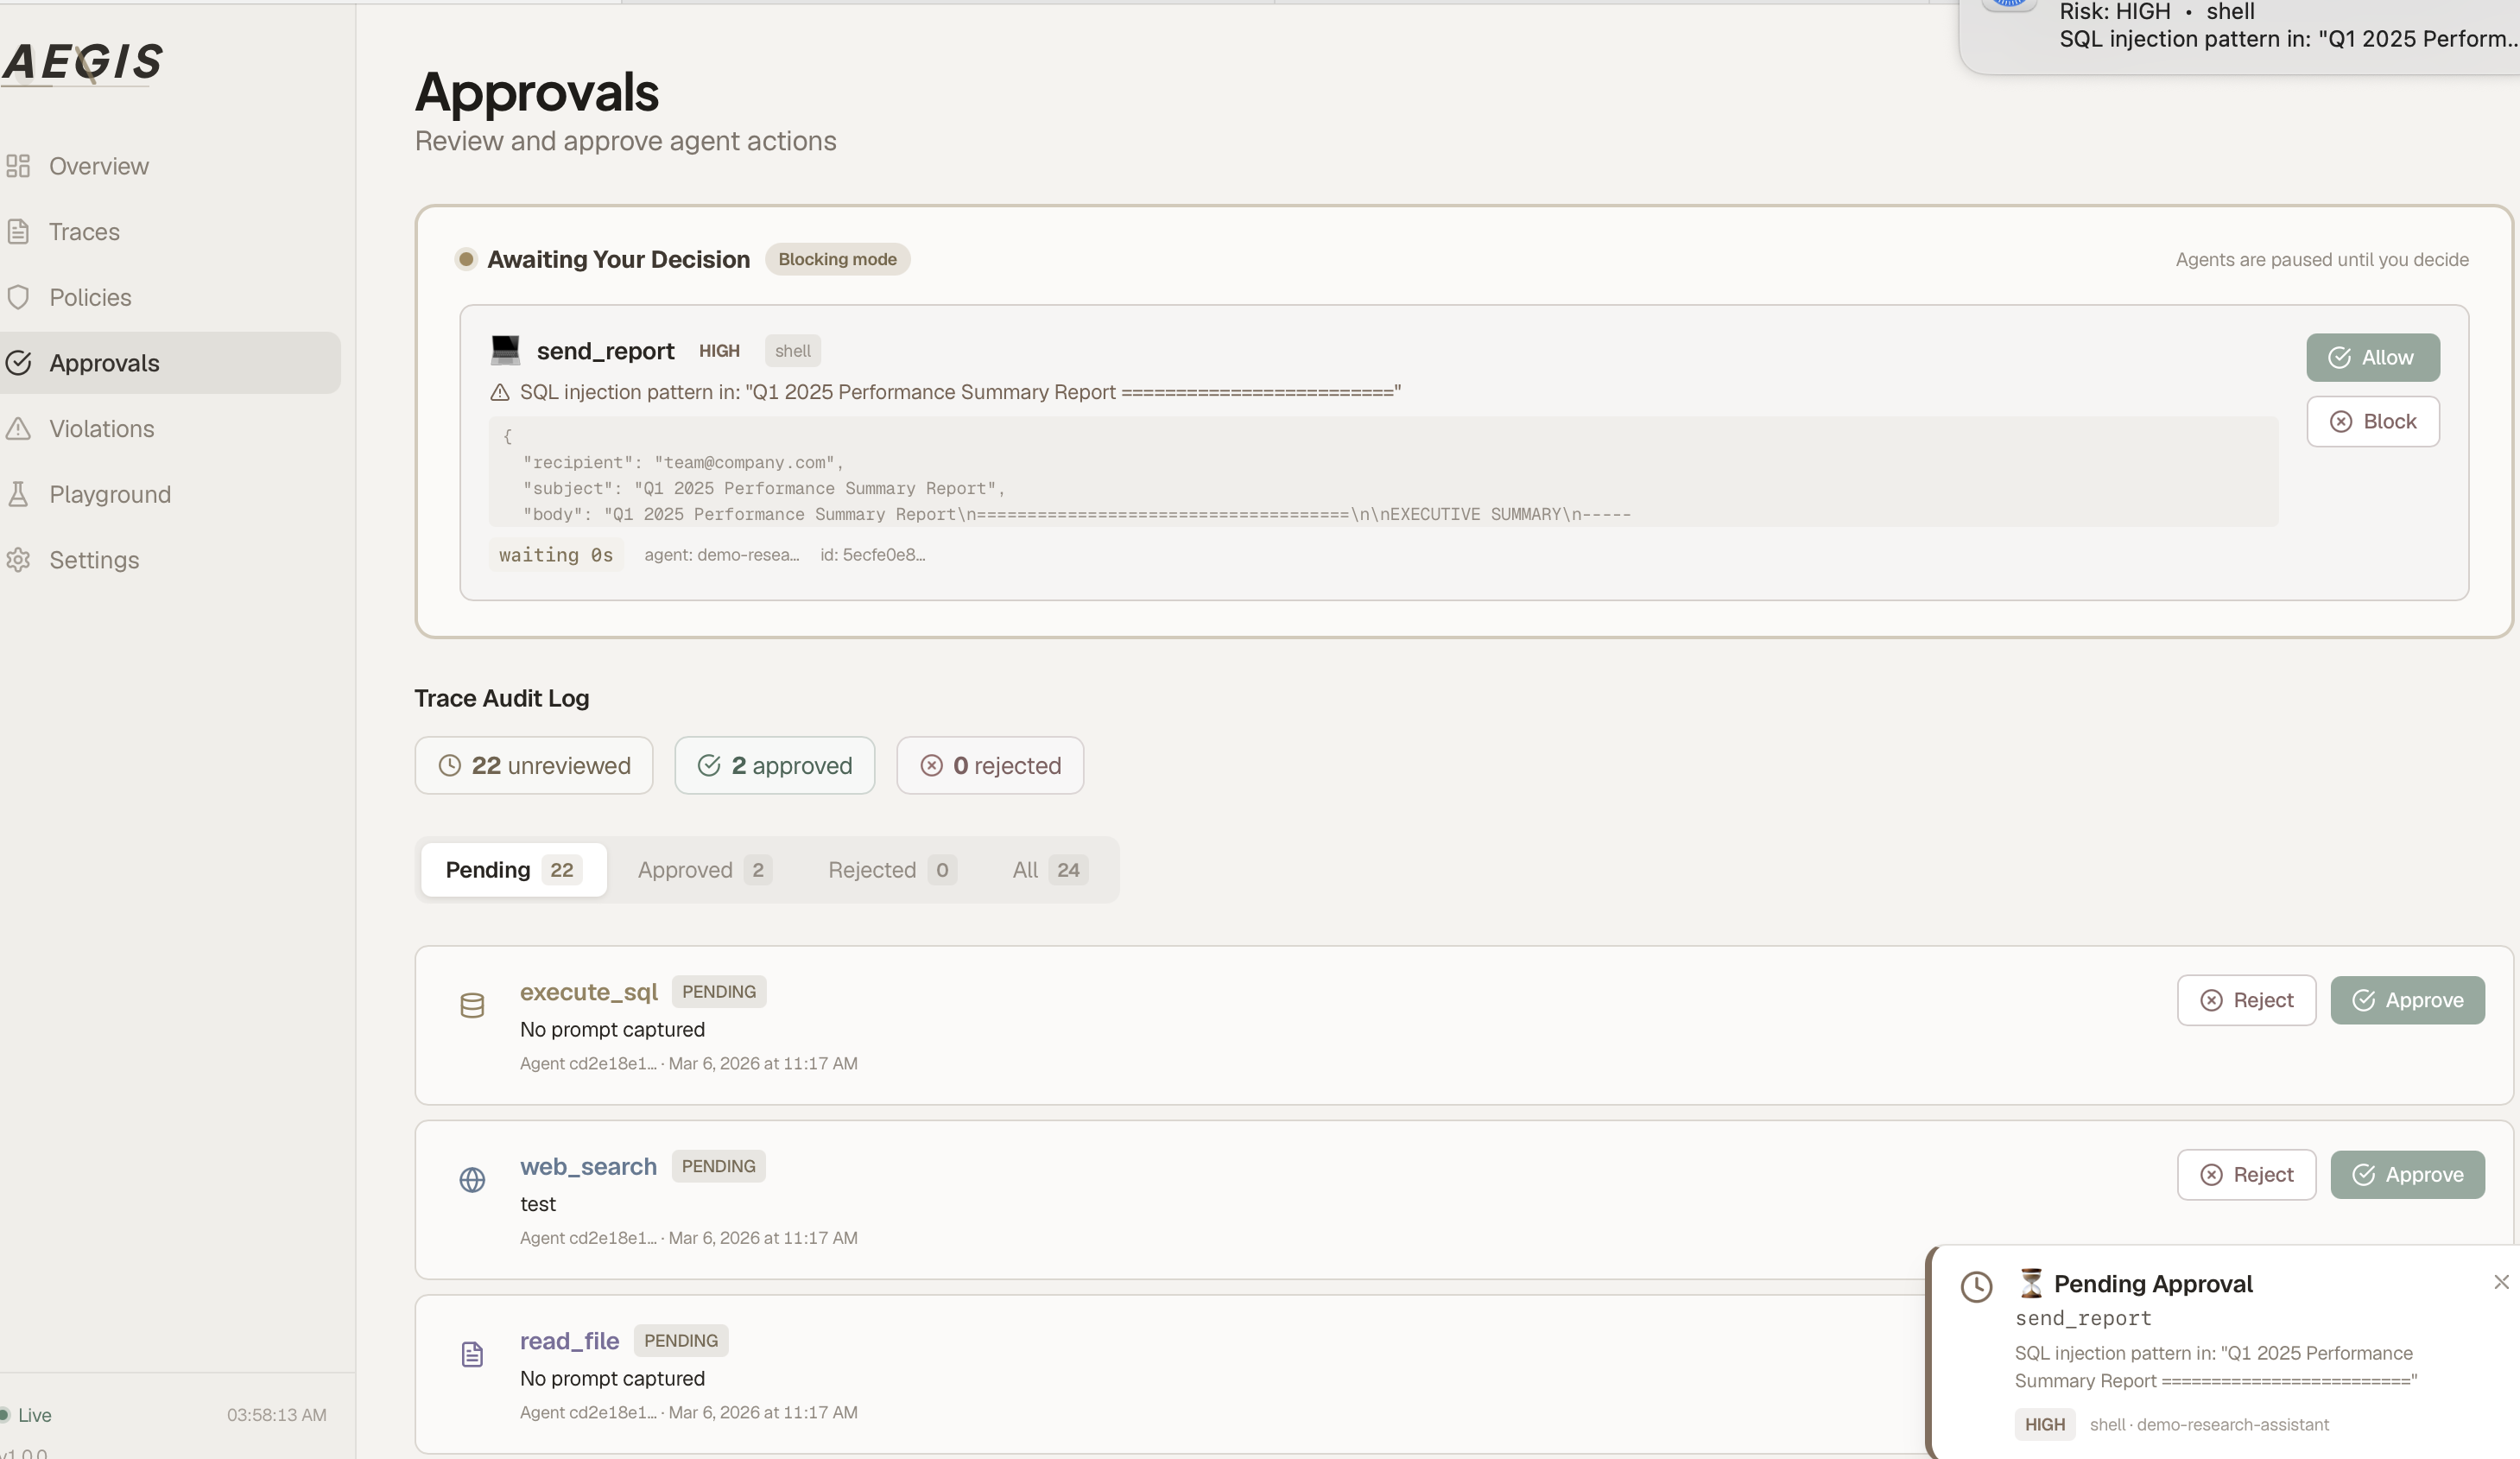
\includegraphics[width=\columnwidth]{images/pending.png}
    \vspace{-0.2in}
    \caption{Human-in-the-loop: a high-risk skill invocation is held pending for reviewer approval.}
    \label{fig:pending-detail}
\end{figure}

\begin{figure}[H]
    \centering
    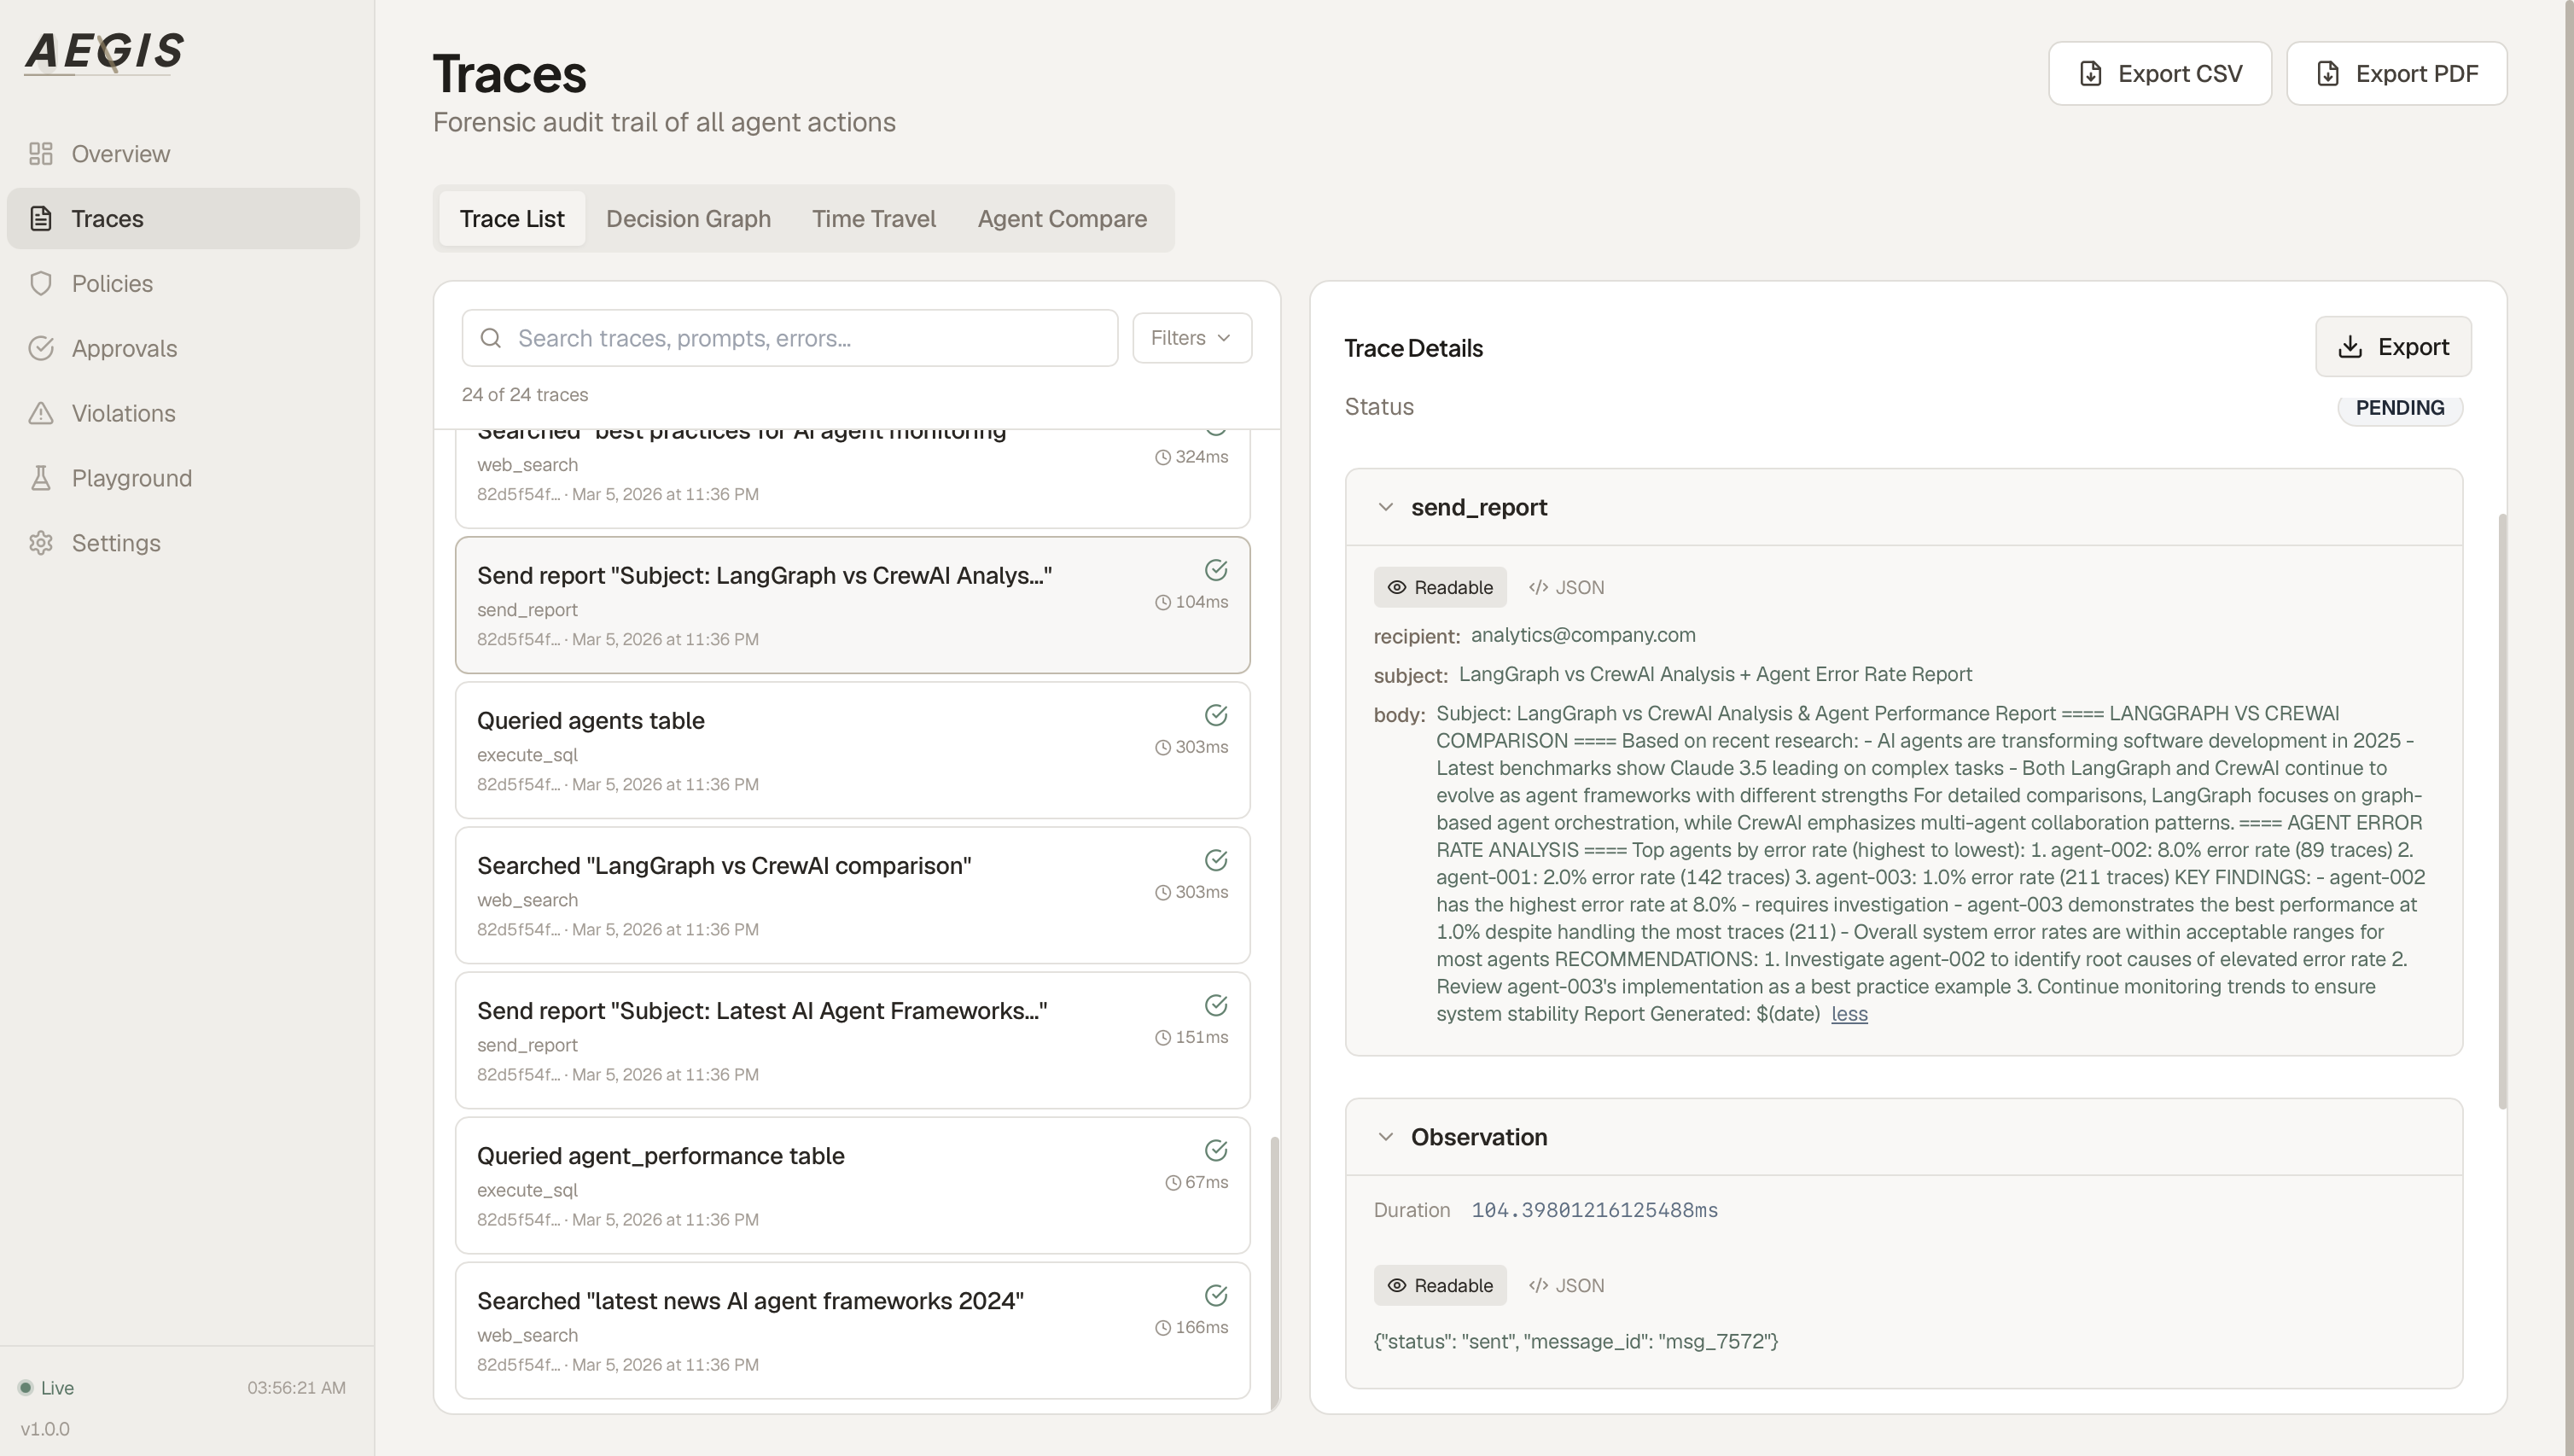
\includegraphics[width=\columnwidth]{images/trace.png}
    \vspace{-0.2in}
    \caption{Forensic trace detail with full arguments, risk signals, classification, and session context.}
    \label{fig:trace-detail}
\end{figure}

\end{document}
